%%%%%%%%%%%%%%%%%%%%%%%%%%%%%%%%%%%%%%%%%%%%%%%%%%%%%%%%%%%%%%%%%%%%%%%%%%%%%%%%
\section{Recovering Shape from Image Collections}\label{sec:imag_coll_problem}
%%%%%%%%%%%%%%%%%%%%%%%%%%%%%%%%%%%%%%%%%%%%%%%%%%%%%%%%%%%%%%%%%%%%%%%%%%%%%%%%
In this section we describe how a spherical harmonic (SH) basis can be recovered
using U-PS techniques. We then describe how this
problem generalises to a multi-person dataset and how a representation of shape
can be recovered per image. Finally, we discuss the importance of achieving
correspondence between the images in an efficient and scalable manner.
%%%%%%%%%%%%%%%%%%%%%%%%%%%%%%%%%%%%%%%%%%%%%%%%%%%%%%%%%%%%%%%%%%%%%%%%%%%%%%%%
\subsection{Spherical Harmonic Bases}\label{subsec:imag_coll_spherical_harmonic}
%%%%%%%%%%%%%%%%%%%%%%%%%%%%%%%%%%%%%%%%%%%%%%%%%%%%%%%%%%%%%%%%%%%%%%%%%%%%%%%%
The Lambertian reflectance model states that matte materials reflect light
uniformly in all directions. This simple image formation model assumes that the
intensity of light reflecting from a surface is a function of the shape of the
surface and a linear combination of point light sources. More formally, given an
image $I(x, y)$, the intensity at a given pixel $(x, y)$ of a convex Lambertian
surface illuminated by a single light, can be expressed as
%%%%%%%%%%%%%%%%%%%
\begin{equation}\label{eq:lambert_law}
    I(x, y) = \rho(x, y) \bb{l}^T \bb{n}(x, y),
\end{equation}
%%%%%%%%%%%%%%%%%%%
where $\rho(x, y)$ is the albedo at the pixel and represents surface
reflectivity, $\bb{l}$ is the vector denoting the single point light source
illuminating the object and $\bb{n}(x, y)$ is the surface normal at the
pixel.

If we now consider a collection of directional light sources placed at infinity,
the lighting intensity at a given pixel can be expressed as a non-negative
function of the unit sphere using a sum of spherical harmonics. Formally,
%%%%%%%%%%%%%%%%%%%
\begin{equation}\label{eq:spherical_harmonics}
    I(x, y) = \sum^{\infty}_{n=0} \sum^{n}_{m=-n} \alpha_n \; \ell_{nm} \; \rho(x,y) \; Y_{nm}(\bb{n}(x,y)),
\end{equation}
%%%%%%%%%%%%%%%%%%%
where $\alpha_n = \pi, 2\pi/3, \pi/4, \ldots$, $\ell_{nm}$ are the coefficients
of the harmonic expansion of the lighting and $Y_{nm}(\bb{n}(x,y))$ are the
surface SH functions evaluated at the surface normal, $\bb{n}(x,y)$. As
$n \rightarrow \infty$, the coefficients tend to zero and thus the SH can be
accurately represented by the lower order harmonics. \citet{frolova2004accuracy}, it
was shown that the first order SH function is guaranteed to represent at least
$87.5\%$ of the reflectance and experimentally verified to recover up to $90\%$
in the case of faces. The first order SH expansion is also directly related to
the objects surface normals:
%%%%%%%%%%%%%%%%%%%
\begin{equation}\label{eq:first_order_spherical_harmonics}
    \begin{aligned}
        \bb{Y}(\bb{n}(x, y))  = \rho(x, y) {[ 1, \bb{n}_{x}(x, y), \bb{n}_{y}(x, y), \bb{n}_{z}(x, y) ]}^T,
   \end{aligned}
\end{equation}
%%%%%%%%%%%%%%%%%%%
where $\bb{n}_{i}(x, y)$ denotes the $i$th component of the normal vector. 
This is a particularly useful result as recovering the first order SH means 
directly recovering a representation of shape for an object.
%%%%%%%%%%%%%%%%%%%%%%%%%%%%%%%%%%%%%%%%%%%%%%%%%%%%%%%%%%%%%%%%%%%%%%%%%%%%%%%%
\subsection{Uncalibrated Photometric Stereo}\label{subsec:imag_coll_uncalibrated_ps}
%%%%%%%%%%%%%%%%%%%%%%%%%%%%%%%%%%%%%%%%%%%%%%%%%%%%%%%%%%%%%%%%%%%%%%%%%%%%%%%%
Classical PS seeks to recover the normals of a convex
object given a number of images under known different lighting conditions. 
Traditionally, the following decomposition is performed
%%%%%%%%%%%%%%%%%%%
\begin{equation}\label{eq:general_ps}
    \bb{X} = \bb{N} \tilde{\bb{L}},
\end{equation}
%%%%%%%%%%%%%%%%%%%
where $\bb{X} \in \bb{R}^{d \times n}$ is the matrix of observations,
and each of the $n$ columns represents a vectorised image of the object with $d$
total pixels, $\bb{N} \in \bb{R}^{d \times 3}$ contains the normal at
every pixel and $\tilde{\bb{L}} \in \bb{R}^{3 \times n}$ is the matrix
of lighting vectors per image. Assuming accurate light vectors and no shadowing
artefacts, this problem is trivially solved as a linear least squares problem.
Photometric stereo has been shown to provide accurate facial reconstructions
despite faces not representing true Lambertian objects. For example, there are
many publicly available facial PS datasets that are discussed in
\cref{subsec:bg_databases} and \cref{sec:bg_ps}.

If the lighting vectors are inaccurate or unknown, then PS is said to be
uncalibrated. \citet{basri2007photometric} showed that $\bb{X}$ can
be decomposed via a rank constrained singular value decomposition (SVD) to
recover the SH bases and the lighting coefficients in the uncalibrated setting.
First order SH are recovered by a rank 4 SVD and are accurate up to a $4 \times 4$ 
generalised Lorentz transformation. By enforcing constraints such as the
integrability constraint~\cite{frankot1988method}, the first order SH, and thus the
normals, can be recovered up to a generalised bas relief ambiguity (GBR).
Formally, uncalibrated PS looks to recover
%%%%%%%%%%%%%%%%%%%
\begin{equation}\label{eq:uncalibrated_ps}
    \bb{X} = \bb{B} \bb{L},
\end{equation}
%%%%%%%%%%%%%%%%%%%
where $\bb{X}$ is as before, $\bb{B} \in \bb{R}^{d \times 4}$ 
contains the first order SH basis images and
$\bb{L} \in \bb{R}^{4 \times n}$ is the matrix of lighting coefficients. 
As previously mentioned, the solution to this problem is found by performing an
SVD,
$\bb{X} =\nobreak \bb{U} \bb{\Sigma} \bb{V}^T$, $\bb{B} = \bb{U} \sqrt{\bb{\Sigma}}$
and $\bb{L} = \sqrt{\bb{\Sigma}} \bb{V}^T$. 
U-PS is useful as it is not always possible to recover accurate 
lighting estimations for every image.
%%%%%%%%%%%%%%%%%%%%%%%%%%%%%%%%%%%%%%%%%%%%%%%%%%%%%%%%%%%%%%%%%%%%%%%%%%%%%%%%
\subsection{Class Specific Uncalibrated Photometric Stereo}\label{subsec:imag_coll_class_uncalibrated_ps}
%%%%%%%%%%%%%%%%%%%%%%%%%%%%%%%%%%%%%%%%%%%%%%%%%%%%%%%%%%%%%%%%%%%%%%%%%%%%%%%%
A generalisation of the U-PS problem for a specific class involves
recovering a joint basis of deformation and illumination. In the case of SH for
faces, this means attempting to separate the identity and deformation of the
individual from the spherical harmonic representation of their face. 
This problem is a classic example of a bilinear
decomposition problem and has been previously studied for use in 3D surface
recovery~\cite{zhou2007appearance,minsik2014realtime,minsik2011fast,%
lee2005bilinear,KemelmacherShlizerman:2013iv}. In
the case of SH, we seek to recover a low dimensional linear subspace that can
recover normals for multiple individuals. This subspace implies that a face can
be accurately reconstructed using a linear combination of basis shapes. This
assumption is commonly employed in algorithms such as the 3DMM and AAMs.
Assuming that we want to recover $k$ such components for our shape subspace, and
that we are using the first order SH, we will recover a $d \times 4k$ basis
matrix that allows us to recover 3D facial shape for multiple individuals.
Formally,
%%%%%%%%%%%%%%%%%%%%%%%%%%
\begin{equation}\label{eq:class_specific_ps}
        \bb{X} = \bb{B} (\bb{L} \ast \bb{C}),
\end{equation}
%%%%%%%%%%%%%%%%%%%%%%%%%%
where $\bb{B} \in \bb{R}^{d \times 4k}$ is the linear basis,
$\bb{L} \in \bb{R}^{4 \times n}$ is the matrix of first order SH lighting
coefficients, $\bb{C} \in \bb{R}^{k \times n}$ is the matrix of shape
coefficients and $(\cdot \ast \cdot)$ denotes the Khatri-Rao
product~\cite{khatri1968solutions}. In fact, this is the exact decomposition problem
solved by \citet{KemelmacherShlizerman:2013iv} where they denote the combined
coefficients matrix as $\bb{P} = \bb{L} \ast \bb{C}$. This was partially
recognised by \citet{zhou2007appearance}, however they recover the lighting and
shape coefficient separately by iteratively solving for each in an alternating
fashion. \citet{zhou2007appearance} also do not provide any examples of the
quality of the shape estimate that they recover.

\citet{minsik2014realtime,minsik2011fast} also attempt this decomposition by
posing the problem in the form of a tensor. The decomposition can then be solved
by applying a multilinear SVD.\@ However, multilinear SVD requires a tensor
representation and thus these techniques require prior data to recover results.
A tensor representation is useful, however, for illustrating how to recover the
$d \times 4$ first order SH for an individual, given their coefficients vector
$\bb{c}_i \in \bb{R}^{k \times 1}$. We reshape the basis matrix
$\bb{B}$ as a tensor which we denote $\bb{S} \in \bb{R}^{d \times k
\times 4}$. The tensor product along the second mode, $\bb{S} \times_2 \bb{c}_i$, 
recovers the person specific shape of the $i$th column of
$\bb{X}$. To recover $\bb{B}$ from $\bb{S}$, we perform
matricisation of $\bb{S}$ along the first mode, denoted $\bb{S}_{(1)}$,
to yield $\bb{S}_{(1)} = \bb{B} \in \bb{R}^{d \times 4k}$.

The problem given in~\eqref{eq:class_specific_ps} can now be minimised using
classic matrix decomposition optimisation frameworks, which we examine in
detail in the next section.
%%%%%%%%%%%%%%%%%%%%%%%%%%%%%%%%%%%%%%%%%%%%%%%%%%%%%%%%%%%%%%%%%%%%%%%%%%%%%%%%
\subsection{Robust Construction Of Spherical Harmonic Bases}\label{subsec:imag_coll_robust_sh_basis}
%%%%%%%%%%%%%%%%%%%%%%%%%%%%%%%%%%%%%%%%%%%%%%%%%%%%%%%%%%%%%%%%%%%%%%%%%%%%%%%%
Inspired by recent advances in robust low-rank subspace
recovery~\cite{candes2011robust}, we seek to modify \cref{eq:class_specific_ps} to
include new constraints that impose robustness to sparse outliers.
As mentioned previously, faces
can be accurately reconstructed by a linear combination of faces taken from a
low-dimensional basis. Therefore, we propose to decompose the image matrix into
a low-rank part ($\bb{A}$) capturing the low frequency shape information and a
sparse part ($\bb{E}$) accounting for gross but sparse noise such as partial
occlusions and pixel corruptions. To promote low-rank and sparsity the nuclear
norm (denote by $\lVert \bb{\cdot} \rVert_{*}$) and the $\ell_1$-norm (denote by
$\lVert \bb{\cdot} \rVert_{1}$) are employed, respectively. Formally we propose
to solve the following non-convex optimisation problem:
%%%%%%%%%%%%%%%%%%%
\begin{equation}
\begin{aligned}
    &\argmin_{\bb{A},\bb{E},\bb{B},\bb{L},\bb{C}} & &\lVert \bb{A} \rVert_{*} + \lambda \lVert \bb{E} \rVert_{1} + \frac{\mu}{2} \lVert \bb{A} - \bb{B} (\bb{L} \ast \bb{C}) \rVert^{2}_{F} \\
    & \text{subject to} & & \bb{X} = \bb{A} + \bb{E}, \; \bb{B}^T \bb{B} = \bb{I}.
\end{aligned}
\label{eq:robust_sh_problem}
\end{equation}
%%%%%%%%%%%%%%%%%%%
Although the above problem is non-convex, an accurate solution can be obtained
by employing the Alternating Directions Method (ADM)~\cite{bertsekas2014constrained}. That
is, to minimise the following augmented Lagrangian function:
%%%%%%%%%%%%%%%%%%%
\begin{equation}
    \begin{aligned}
        \mathcal{L}(\bb{A},\bb{E},\bb{B},\bb{C},\bb{L},\bb{Y}) &= \lVert \bb{A} \rVert_{*} + \lambda \lVert \bb{E} \rVert_{1} + \frac{\mu}{2} \lVert \bb{A} - \bb{B} (\bb{L} \ast \bb{C}) \rVert^{2}_{F} \quad + \\
        & \quad \Tr{(\bb{Y}^T(\bb{X} - \bb{A} - \bb{E}))} +  \frac{\mu}{2} \lVert \bb{X} - \bb{A} - \bb{E} \rVert_{F}^{2},
    \end{aligned}\label{eq:augmented_lagrangian}
\end{equation}
%%%%%%%%%%%%%%%%%%%
with respect to $\bb{B}^T \bb{B} = \bb{I}$. Let $t$ denote the iteration index. 
Given $\bb{A}_{[t]}$, $\bb{E}_{[t]}$, $\bb{B}_{[t]}$, $\bb{C}_{[t]}$, $\bb{L}_{[t]}$, $\bb{Y}_{[t]}$
and $\mu_{[t]}$, the iteration of ADM for \cref{eq:robust_sh_problem} reads:
%%%%%%%%%%%%%%%%%%%
\begin{align}
    \bb{A}_{[t+1]} &= \lVert \bb{A}_{[t]} \rVert_{*} + \frac{\mu_{[t]}}{2} \biggl( \lVert \bb{A}_{[t]} - \bb{B}_{[t]} (\bb{L}_{[t]} \ast \bb{C}_{[t]}) \rVert^{2}_{F} + \lVert \bb{X} - \bb{A}_{[t]} - \bb{E}_{[t]} + \frac{\bb{Y}_{[t]}}{\mu_{[t]}} \rVert_{F}^{2} \biggr), \label{eq:text_A_update} \\
    \bb{E}_{[t+1]} &= \argmin_{\bb{E}_{[t]}} \lambda \lVert \bb{E}_{[t]} \rVert_{1} + \frac{\mu_{[t]}}{2} \lVert \bb{X} - \bb{A}_{[t+1]} - \bb{E}_{[t]} + \frac{\bb{Y}_{[t]}}{\mu_{[t]}} \rVert_{F}^{2}, \label{eq:text_E_update} \\
    \bb{B}_{[t+1]} &= \argmin_{\bb{B}_{[t]}^T \bb{B}_{[t]} = \bb{I}} \frac{\mu_{[t]}}{2} \lVert \bb{A}_{[t+1]} - \bb{B}_{[t]} (\bb{L}_{[t]} \ast \bb{C}_{[t]}) \rVert_{F}^{2}, \label{eq:text_B_update} \\
    \left[ \bb{L}_{[t+1]}, \bb{C}_{[t+1]} \right] &= \argmin_{\bb{L}_{[t]}, \bb{C}_{[t]}} \frac{\mu_{[t]}}{2} \lVert \bb{A}_{[t+1]} - \bb{B}_{[t+1]} (\bb{L}_{[t]} \ast \bb{C}_{[t]}) \rVert_{F}^{2}. \label{eq:text_LC_update}
\end{align}
%%%%%%%%%%%%%%%%%%%
Sub-problem~\eqref{eq:text_A_update} admits a closed-form solution, given by the
singular value thresholding (SVT)~\cite{cai2010singular} operator as:
%%%%%%%%%%%%%%%%%%%
\begin{equation}\label{eq:text_A_SVT}
    \bb{A}_{[t+1]} = D_{\mu_{[t]}^{-1}} \left[ \bb{M}_{[t]}  - \bb{A}_{[t]} + \bb{X} - \bb{E}_{[t]} + \frac{\bb{Y}_{[t]}}{\mu_{[t]}} \right],
\end{equation}
%%%%%%%%%%%%%%%%%%%
where $\bb{M}_{[t]} = \bb{B}_{[t]} (\bb{L}_{[t]} \ast \bb{C}_{[t]})$ is introduced 
for brevity of the equation and the SVT is defined as
$D_{\tau}(\bb{Q}) = \bb{U} \bb{S}_{\tau} \bb{V}^T$ for any matrix $\bb{Q}$ with SVD:\@
$\bb{Q} = \bb{U} \bb{S} \bb{V}^T$. 
Subp-roblem~\eqref{eq:text_E_update} has a unique solution that is obtained via 
the element-wise shrinkage operator~\cite{candes2011robust}. The shrinkage operator 
is defined as $\mathcal{S}_{\tau}[q]=\mbox{sgn}(q) \: \max(|q|-\tau, 0)$. 
Therefore, the solution of~\eqref{eq:text_E_update} is
%%%%%%%%%%%%%%%%%%%
\begin{equation}\label{eq:text_E_shrinkage}
    \bb{E}_{[t+1]} = \mathcal{S}_{\lambda \mu_{[t]}^{-1}} \left[ \bb{X} - \bb{A}_{[t+1]} + \frac{\bb{Y}_{[t]}}{\mu_{[t]}} \right].
\end{equation}
%%%%%%%%%%%%%%%%%%%
{ % Courtesy of the wonderful 4G!
%%%%%%%%%%%%%%%%%%%
\def\t#1{{\bb{#1}_{[t]}}}
\def\tp#1{{\bb{#1}_{[t+1]}}}
%%%%%%%%%%%%%%%%%%%
\noindent Sub-problem~\eqref{eq:text_B_update} is a reduced rank Procrustes
Rotation problem~\cite{zou2006sparse}. Its solution is given by
$\bb{B}_{[t]} = \bb{U} \bb{V}^{\top}$ with
%%%%%%%%%%%%%%%%%%%
\begin{equation}\label{eq:text_B_update2}
    \tp A {\left(\t L \ast \t C\right)}^{\top} = \bb{U} \bb{\Sigma} \bb{V^{\top}},
\end{equation} 
%%%%%%%%%%%%%%%%%%%
being the SVD of $\tp A {\left(\t L \ast \t C\right)}^{\top}$. However, due the
unitary invariance of the Frobenius norm, Equation~\ref{eq:text_LC_update}
becomes
%%%%%%%%%%%%%%%%%%%
\begin{equation}\label{eq:text_LC_update2}
    \argmin_{\bb{L}_{[t+1]}, \bb{C}_{[t+1]}} \lVert \bb{B}_{[t+1]}^T\bb{A}_{[t+1]} - \bb{L}_{[t]} \ast \bb{C}_{[t]} \rVert_{F}^{2}.
\end{equation}
%%%%%%%%%%%%%%%%%%%
Sub-problem~(\ref{eq:text_LC_update},~\ref{eq:text_LC_update2}) is a least 
squares factorisation of a Khatri-Rao product~\cite{roemer2010tensor}, which is 
solved as follows:
Let $\bb{Q} = \tp B^{\top} \tp A, \bb{L} = \t L, \text{and} \; \bb{C} = \t C$. 
Furthermore, let $\bb{q}_i, \bb{l}_i, \text{and} \; \bb{c}_i$ be the $i_{th}$ 
columns of 
matrices $\bb{Q}, \bb{L}, \text{and} \; \bb{C}$, respectively. 
Clearly $\bb{q}_i = \bb{l}_i \oplus \bb{c}_i$, where $\oplus$ denotes the Kronecker 
product. For each column of $\bb{Q}$: Reshape $\bb{q}_i$ into a 
matrix $\tilde{\bb{Q}}_i \in \bb{R}^{4 \times k}$ 
such that 
$\text{vec}\left(\tilde{\bb{Q}}_i\right) = \bb{q}_i$. 
Obviously, $\tilde{\bb{Q}}_i = \bb{c}_i \cdot {\bb{l}_i}^{\top}$ is a rank-one matrix.
Compute the SVD of
$\tilde{\bb{Q}}_i$ as $\tilde{\bb{Q}}_i = \bb{U}_i \bb{\Sigma}_i {\bb{V}_i}^{\top}$. 
The best rank-one approximation of $\tilde{\bb{Q}}_i$ is obtained by truncating the SVD as:
$\bb{l}_i = \bb{u}_i \sqrt{\sigma_1}$ and $\bb{c}_i = \sqrt{\sigma_1} \bb{v}_i$,
where $\bb{u}_i$ and $\bb{v}_i$ are the first column vectors of $\bb{U}_i$
and $\bb{V}_i$, respectively, and $\sigma_1$ is the largest singular value.
The ADM for solving~\eqref{eq:robust_sh_problem} is outlined in 
\cref{alg:imag_coll_adm_solution}.
}

It is important to note that there are inherent ambiguities in this
decomposition, both from the SVD to recover $\bb{B}$ and in the Khatri-Rao
factorisation to recover $\bb{L}$ and $\bb{C}$. In particular, we are most
concerned about how they may affect the recovered normals before we integrate
them to recover depth. In order to resolve these ambiguities, we take the
simplest possible approach, we resolve the ambiguity using a template set
of normals provided by a known mean face.
%%%%%%%%%%%%%%%%%%%%%%%%%%%%%%%%%%%%%%%%%%%%%%%%%%%%%%%%%%%%%%%%%%%%%%%%%%%%%%%%
%%%%%%%%%%%%%%%%%%%%%%%%%%%%%%%%%%%%%%%%%%%%%%%%%%%%%%%%%%%%%%%%%%%%%%%%%%%%%%%%
\begin{algorithm}[t]
    \caption{Solving~\eqref{eq:robust_sh_problem} by the ADM method.}
\label{alg:adm_solution}
    {\scriptsize\textbf{Input:} Data Matrix $\bb{X} \in \mathbb{R}^{d \times n}$ and parameter $\lambda$.} \\
    {\scriptsize\textbf{Output:} Matrices $\bb{A}$, $\bb{E}$, $\bb{B}$, $\bb{C}$, $\bb{L}$.}  \\
{
    \scriptsize
    % Define commands
    \def\At{{\bb{A}_{[t]}}}
    \def\Et{{\bb{E}_{[t]}}}
    \def\Ct{{\bb{C}_{[t]}}}
    \def\Lt{{\bb{L}_{[t]}}}
    \def\Bt{{\bb{B}_{[t]}}}
    \def\Yt{{\bb{Y}_{[t]}}}
    \def\mut{{\mu_{[t]}}}
    \def\X{{\bb{X}}}
    
    \begin{algorithmic}
        \State{}Initialise: $\bb{A}_{[0]} = 0$, $\bb{E}_{[0]} = 0$, $\bb{B}_{[0]} = 0$, $\bb{C}_{[0]} = 0$, $\bb{L}_{[0]} = 0$, $\bb{Y}_{[0]} = 0$, $\mu_{[0]} = 10^{-6}$, $\rho = 1.1$, $\epsilon = 10^{-8}$
        \While{not converged} %(Outer loop)
            \State{}Fix $\Et$, $\Bt$, $\Ct$, $\Lt$ and update $\bb{A}_{[t + 1]}$ by
                \begin{equation}\label{eq:A_update}
                    \bb{A}_{[t+1]} = D_{\mu_{[t]}^{-1}} \left[  \Bt ( \Lt \ast \Ct ) - \At + \X - \Et + \frac{\Yt}{\mut} \right]
                \end{equation}
            \State{}Fix $\bb{A}_{[t+1]}$, $\Lt$, $\Ct$, $\Lt$ and update $\bb{A}_{[t + 1]}$ by
                \begin{equation}\label{eq:E_update}
                    \bb{E}_{[t+1]} = \mathcal{S}_{\lambda \mut^{-1}} \left[ \X - \bb{A}_{[t+1]} + \frac{\Yt}{\mut} \right]
                \end{equation}
            \State{}Update $\bb{B}_{[t+1]}$ by first performing the SVD on:
                \begin{equation}\label{eq:ALC_svd}
                    \bb{A}_{[t+1]} {(\Lt \ast \Ct)}^T = \bb{U} \bb{\Sigma} \bb{V}, \; \bb{B}_{[t+1]} = \bb{U} \bb{V}^T
                \end{equation}
            \State{}Update $[\bb{L}_{[t+1]}, \bb{C}_{[t+1]}]$ via a Least Squares Khatri-Rao factorization, as described in \cref{subsec:robust_sh_basis}
            \State{} Update Lagrange multipliers by
                \begin{equation}\label{eq:Y_update}
                    \bb{Y}_{[t+1]} = \Yt + \mut \left( \X - \bb{A}_{[t+1]} - \bb{E}_{[t+1]} \right)
                \end{equation}
            \State{}Update $\mu_{[t+1]}$ by $\mu_{[t+1]} = \min(\rho \mut, 10^6)$
            \State{}Check convergence condition
                \begin{equation}\label{eq:convergence_condition}
                    \begin{aligned}
                        &\lVert \X - \bb{A}_{[t+1]} - \bb{E}_{[t+1]} \rVert_{\infty} < \epsilon, \\
                        &\lVert \bb{A}_{[t+1]} - \bb{B}_{[t+1]} - (\bb{L}_{[t+1]} \ast \bb{C}_{[t+1]}) \rVert_{\infty} < \epsilon
                    \end{aligned}
                \end{equation}
            \State{}$t \leftarrow t + 1$
        \EndWhile{}
    \end{algorithmic}
}
\end{algorithm}
%%%%%%%%%%%%%%%%%%%%%%%%%%%%%%%%%%%%%%%%%%%%%%%%%%%%%%%%%%%%%%%%%%%%%%%%%%%%%%%%
%%%%%%%%%%%%%%%%%%%%%%%%%%%%%%%%%%%%%%%%%%%%%%%%%%%%%%%%%%%%%%%%%%%%%%%%%%%%%%%%
%%%%%%%%%%%%%%%%%%%%%%%%%%%%%%%%%%%%%%%%%%%%%%%%%%%%%%%%%%%%%%%%%%%%%%%%%%%%%%%%
\subsection{Efficient Pixel-wise Correspondence}\label{subsec:imag_coll_correspondence}
%%%%%%%%%%%%%%%%%%%%%%%%%%%%%%%%%%%%%%%%%%%%%%%%%%%%%%%%%%%%%%%%%%%%%%%%%%%%%%%%
In contrast to the related work of \citet{KemelmacherShlizerman:2013iv},
we achieved pixel-wise correspondence between our images by using existing,
efficient sparse facial alignment algorithms. This has two distinct advantages.
Firstly, recent facial alignment algorithms such as those by
\citet{ren2014face} and \citet{kazemi2014one} can produce a very accurate set
of sparse facial features in the order of a single millisecond. In contrast, the
optical flow method cited in \citet{KemelmacherShlizerman:2013iv} takes multiple
seconds even for a small image. This means that our training time is drastically
reduced in comparison to \citet{KemelmacherShlizerman:2013iv}. 
Ideally, our technique would be able to scale
to the magnitude of thousands of images, whereas the alignment of
\citet{KemelmacherShlizerman:2013iv} would quickly become infeasible as the
number of images increases. In fact, the optical flow step is run multiple times as the
collection flow algorithm is used~\cite{kemelmacher2012collection} which involves an
iterative algorithm of rank 4 decompositions and repeated optical flow.
Secondly, the use of a direct alignment to a single reference frame enables the
the usage of our basis in existing appearance based facial alignment algorithms
such as AAMs. This means that our basis can be used to reconstruct dense 3D
shape of faces directly from an existing AAM fitting provided the reference
space of the AAM and our subspace is the same.
%%%%%%%%%%%%%%%%%%%%%%%%%%%%%%%%%%%%%%%
\begin{figure*}
    \centering
    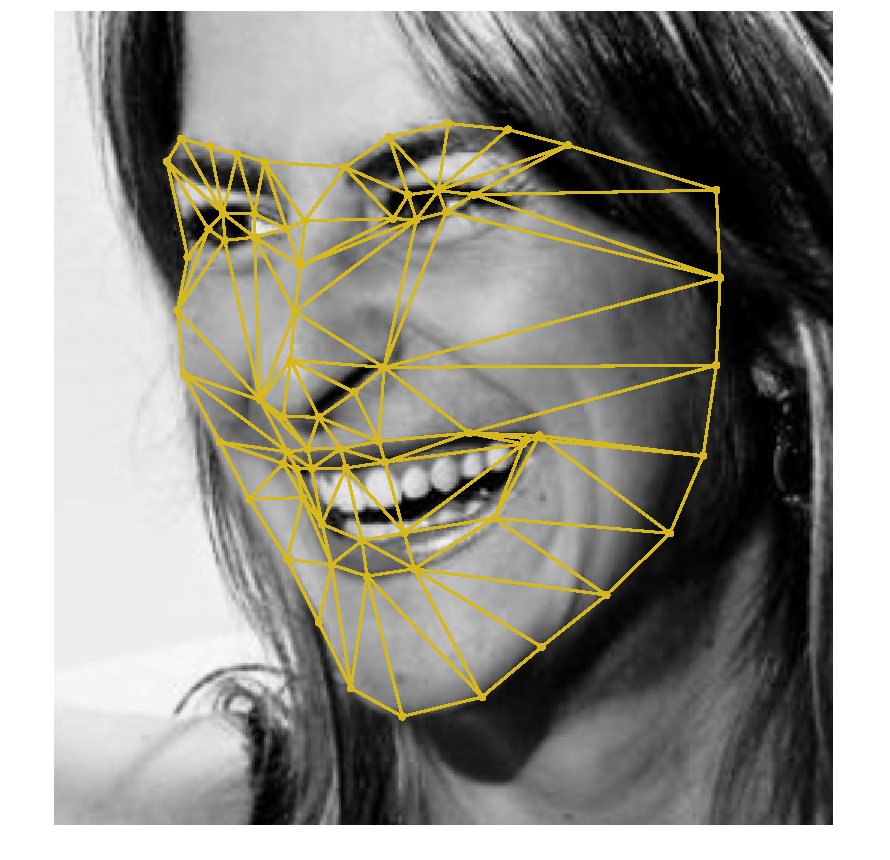
\includegraphics[width=4cm]{collection_ps/images/example_warped_original}
    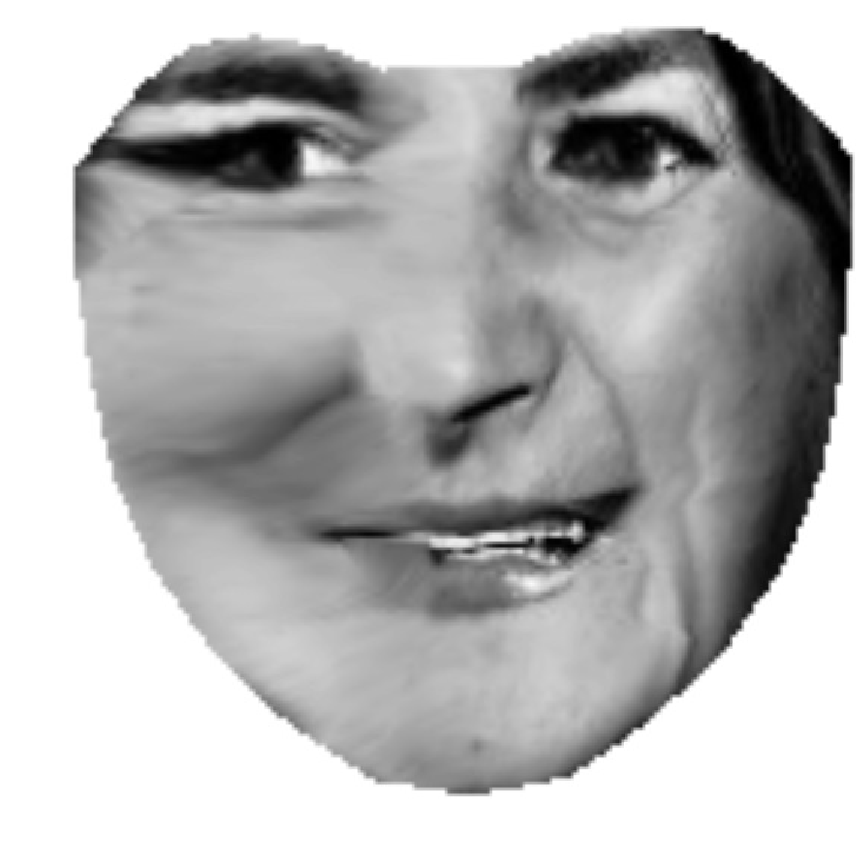
\includegraphics[width=4cm]{collection_ps/images/example_warped}
    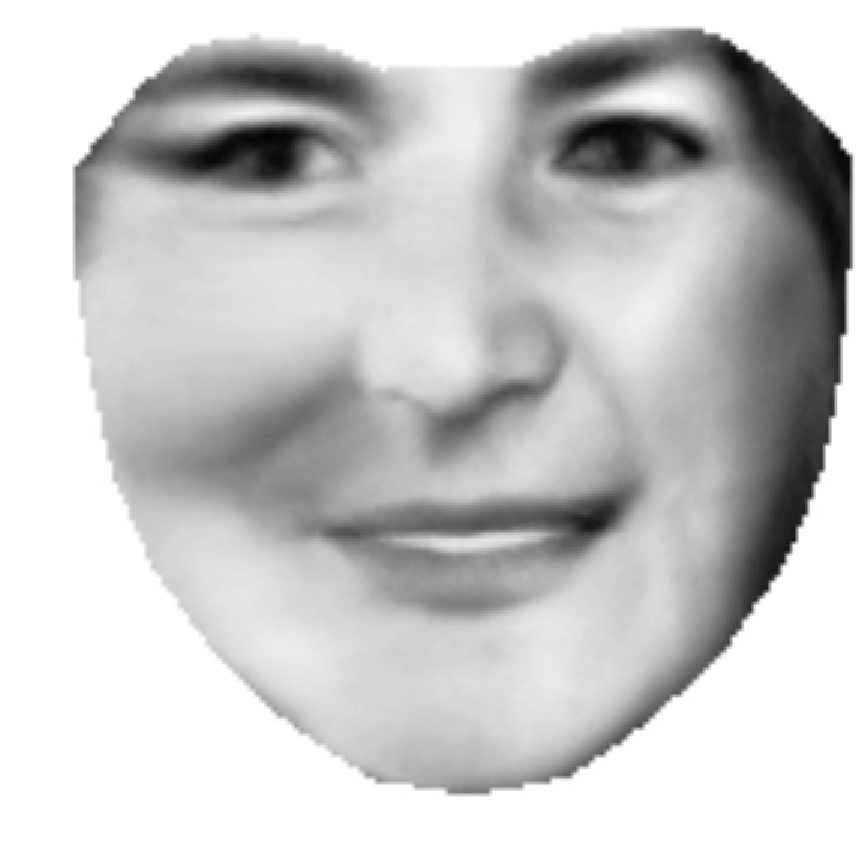
\includegraphics[width=4cm]{collection_ps/images/example_warped_low_rank}
    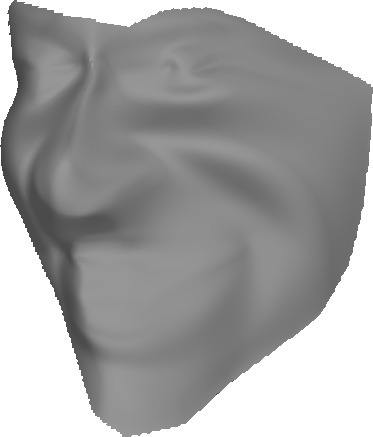
\includegraphics[width=3.8cm,height=3.8cm,trim = 0cm -1cm 0cm 0cm]{collection_ps/images/example_warped_shape}
    \caption{{\bf Example of the low rank effect on warped pose}. From left to
             right: initial input image, input image after warping,
             warped image after the low rank constraint, 
             recovered depth from warped image.}
\label{fig:imag_coll_low_rank_warping}
\end{figure*}
%%%%%%%%%%%%%%%%%%%%%%%%%%%%%%%%%%%%%%%

However, it is important to note that there are two potential drawbacks to our
alignment technique. The alignment is based on a Piecewise Affine warping and is
thus much coarser than the optical flow technique used in \citet{KemelmacherShlizerman:2013iv}.
This is particularly amplified when larger poses are present in the input
images. However, this is partly why the low rank component of our algorithm is
so important. As \cref{fig:imag_coll_low_rank_warping} shows, the robust
decomposition of the basis helps correct these large global errors so that the
shape subspace can be successfully recovered. Secondly, our technique does not
contain a number of sub-clusters that can be used to warp expression onto our
model. However, by using a large number of images that contain expression we
directly include expression within our subspace. 
In \citet{KemelmacherShlizerman:2013iv}, the
recovered subspace will necessarily be devoid of expression as the global
reference shape is neutral. This means that the subspace recovered by
\citet{KemelmacherShlizerman:2013iv} will not be able to recover
expressive 3D shape using efficient facial alignment algorithms.
